\section{结论与展望}
\label{sec:sum}

在本工作中，我们提出了一种利用 ML 社区中流行的扩散模型生成量子场组态的新方法。我们着重指出了它与随机量化（SQ）的联系——后者基于沿虚构时间方向的随机过程来量子化场论。在 SQ 中，随机过程的漂移项是已知的，因为它由希望抽样的概率分布导出，而该分布由所考虑的量子理论决定。在 DMs 中，漂移项未知，而是在前向随机过程中从数据学得。估计出漂移项之后，训练好的 DM 沿相反方向运行，从噪声中创造出独立组态，即``去噪''过程。这后半部分类似于 SQ 中的动力学，只是漂移项是学得的且随时间变化。{在图~\ref{fig:flow-chart} 中，我们以示意方式总结了随机量化与扩散模型之间的关系。}

%%%%%%%%%%%%%%%%%%%%%%%%%%%%%%%%%%%%%%%%%%%%%%%%%%%%%%%%%%%%%%%%%%%%%%%%%%%%%%%%%%%%%%%%%%%%%%%%%%%%%%%%%%%%%%%%%%
\begin{figure}[hbtp!]
    \centering
    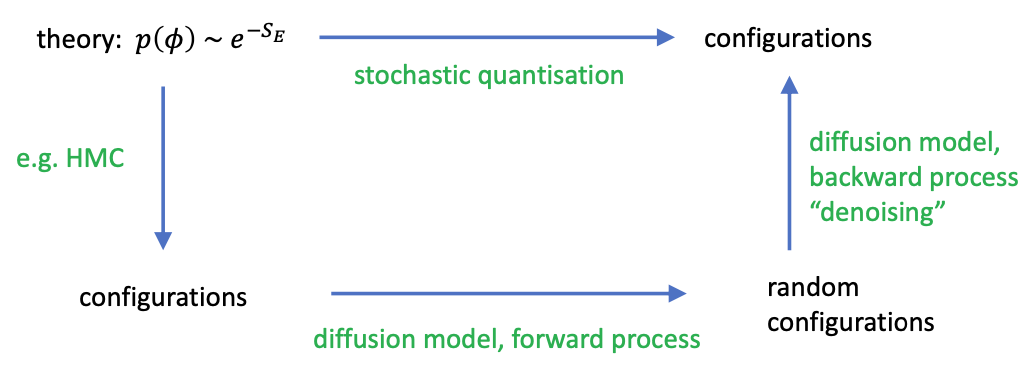
\includegraphics[width = 0.7 \textwidth]{images/flow-chart.png}
    \caption{格点场论情形下随机量化与扩散模型之间关系的示意图。}
    \label{fig:flow-chart}
\end{figure}
%%%%%%%%%%%%%%%%%%%%%%%%%%%%%%%%%%%%%%%%%%%%%%%%%%%%%%%%%%%%%%%%%%%%%%%%%%%%%%%%%%%%%%%%%%%%%%%%%%%%%%%%%%%%%%%%%%

我们在一个简单玩具模型以及具有 $\phi^4$ 相互作用的二维标量场论（对称相与破缺相皆备）中演示了该方法。我们证明 DM 可以充当全局采样器来辅助基于蒙特卡洛原理的方法。我们指出，可以在每条轨迹的末尾加入接受--拒绝步骤。数值结果表明，训练良好的 DM 能成功复现两个相中的组态，且沿马尔可夫链的自关联时间被缩短。这种采样效率的提升对格点场论研究有益，值得进一步分析。

未来有多个方向可以探索。前向（``光滑化''）与后向（``去噪''）过程令人联想到（逆）重整化群变换，将其精确化将是有趣的工作。
由于作用量可以被相对准确地估计，在不制备训练数据集的情况下训练 DM 是可行的，这有待研究。
DMs 与 SQ 的联系提供了新的视角。人们熟知如何在非阿贝尔规范理论中实施 SQ；因此应当可以为非阿贝尔情形表述 DMs。一个引人入胜的方向是：设想已经为某个含费米子的量子理论（如 QCD 或 Schwinger 模型）生成了一组组态。由于费米子已被``积掉''（integrated out），组态仅由规范场给出。把这些组态作为 DM 的起点，便可以学到隐式纳入费米子效应的有效随机过程。这可用于以数值上``廉价''的方式创造额外组态。还可以加入基于底层理论的接受--拒绝步骤，但这需要计算费米子行列式。最后，SQ 也可用于带符号问题或复作用量问题的理论，即分布非正定的情形，这通常称为复朗之万（CL）动力学。众所周知，CL 在随机过程的长轨迹上可能变得不可靠。把 CL 与 DMs 结合，可以考虑相当短的轨迹，随后用所得组态训练 DM 以生成更多组态来提高统计量。


\section*{致谢}

感谢 Tetsuo Hatsuda、Shuzhe Shi 与 Xu-Guang Huang 教授的有益讨论。
感谢 ECT* 以及位于达姆施塔特 GSI 的 ExtreMe Matter Institute EMMI 在本文撰写期间（2023 年 6 月）举办的 ECT*/EMMI 研讨会 {\em Machine learning for lattice field theory and beyond} 期间的支持。
本工作得到：(i) 香港中文大学（深圳）大学发展基金（No. UDF01003041）与 ErUM-Data 行动计划中 BMBF 资助的 KISS 联盟（05D23RI1）（K.Z.）；(ii) SAMSON AG 的 AI 基金（法兰克福）（K.Z. 与 L.W.）；(iii) 西电-FIAS 国际联合研究中心（L.W.）；(iv) STFC Consolidated Grant ST/T000813/1（G.A.）。K.Z. 还感谢 NVIDIA Corporation 捐赠的 NVIDIA GPU。L.W. 还感谢国家自然科学基金（Grant No.12147101）在其访问复旦大学期间为计算资源提供的支持。

\paragraph{补充说明。}近期相关工作将随机过程引入混合蒙特卡洛算法~\cite{Robnik:2023pgt}，并探讨了基于热方程的精确重整化群（ERG）与 DMs 的对应关系~\cite{Cotler:2023lem}。
